\documentclass[a4paper,man,floatsintext,longtable,noextraspace,12pt]{apa6}

\usepackage[english]{babel}
\usepackage[utf8x]{inputenc}
\usepackage{amsmath}
\usepackage{graphicx}
\usepackage[colorinlistoftodos]{todonotes}
\usepackage{hyperref}

\usepackage{booktabs}
\usepackage{longtable}
\usepackage{array}
\usepackage{multirow}
\usepackage{wrapfig}
\usepackage{float}
\usepackage{colortbl}
\usepackage{pdflscape}
\usepackage{tabu}
\usepackage{threeparttable}
\usepackage{threeparttablex}
\usepackage[normalem]{ulem}
\usepackage{makecell}
\usepackage{xcolor}
% make captions italic

% number lines
% \usepackage{lineno}
% \linenumbers
            
% bibliography
\newlength{\cslhangindent}
\setlength{\cslhangindent}{1.5em}
\newenvironment{CSLReferences}%
  {}%
  {\par}

% tightlist
\providecommand{\tightlist}{%
  \setlength{\itemsep}{0pt}\setlength{\parskip}{0pt}}

\title{\textbf{How open are hybrid journals included in transformative agreements?}}
\shorttitle{Hybrid OA}
\author{Najko Jahn}
\affiliation{Göttingen State and University Library, University of Göttingen\\
Platz der Göttinger Sieben 1, 37073 Göttingen, Germany\\
najko.jahn@sub.uni-goettingen.de
}

%\authornote{Correspondence concerning this article should be addressed to Najko Jahn}

\abstract{}

\begin{document}
\maketitle

% QSS wants numbered sections
%\setcounter{secnumdepth}{2}

\hypertarget{introduction}{%
\section{Introduction}\label{introduction}}

\hypertarget{methods-and-data}{%
\section{Methods and data}\label{methods-and-data}}

This study combines data from multiple publicly available data sources
as visualised in Figure 1. Transformative agreement data retrieved from
the cOAlition S Journal Checker Tool provided information about journal
portfolios and participating institutions. After identification of
hybrid journals, Crossref served as the primary data source for
article-level metadata including Creative Commons (CC) license
information to determine open access articles on publisher websites.
OpenAlex provided first author affiliation metadata that were
subsequently linked to the transformative agreement data to identify
open access articles published through these agreements.

\begin{figure}

{\centering 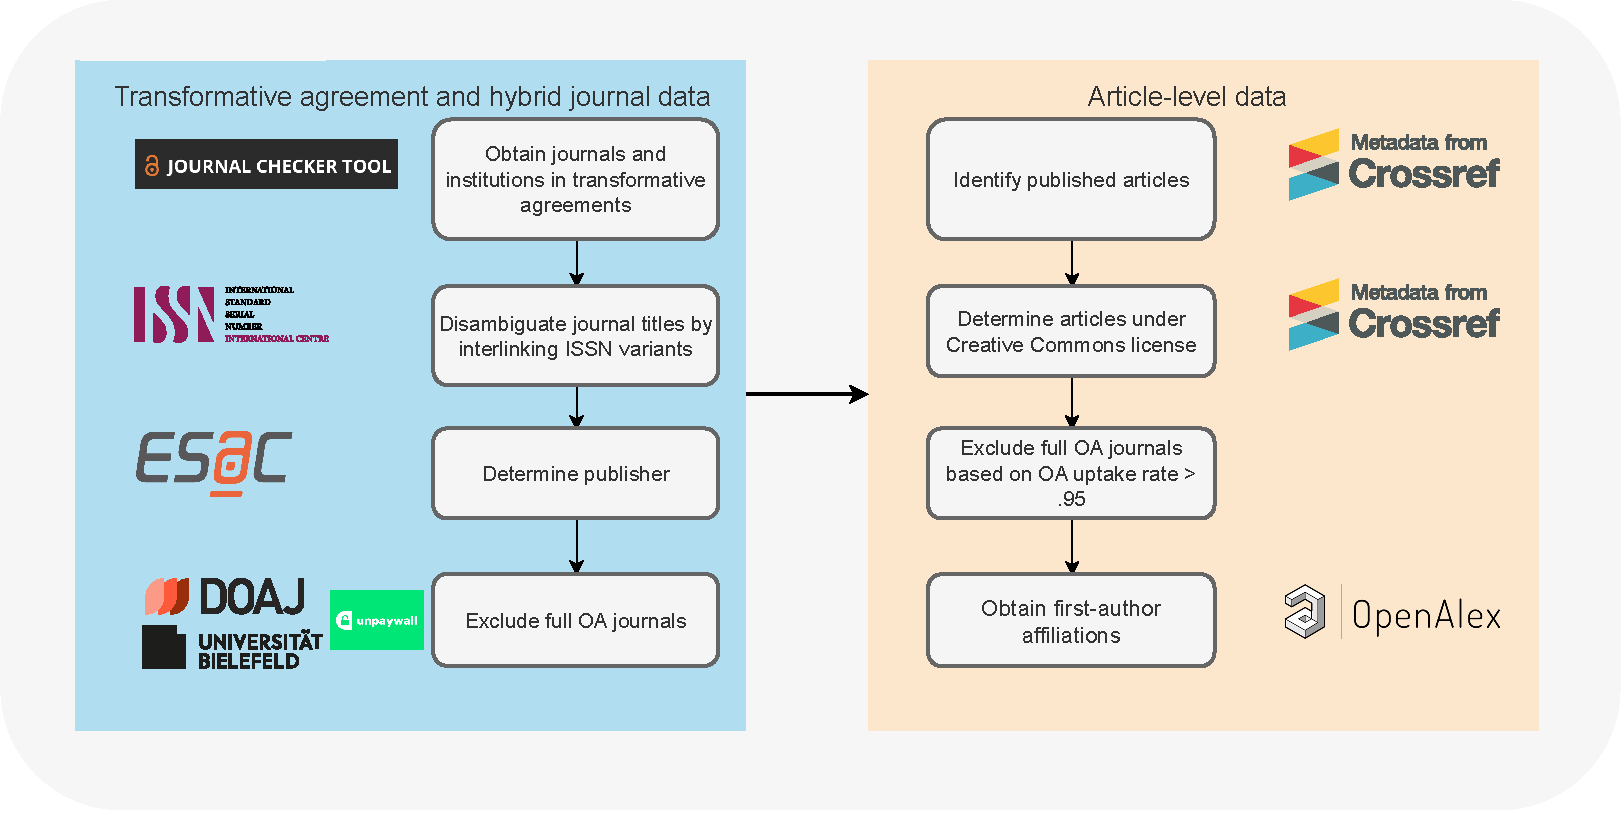
\includegraphics[width=0.99\linewidth]{data_collection_workflow} 

}

\caption{Data collection workflow to obtain article-level transformative agreement data}\label{fig:data_workflow}
\end{figure}

\hypertarget{transformative-agreement-and-hybrid-journal-data}{%
\subsection{Transformative agreement and hybrid journal
data}\label{transformative-agreement-and-hybrid-journal-data}}

Data gathering started with obtaining journals included in
transformative agreements using the publicly available Transformative
Agreement Data dump\footnote{\url{https://journalcheckertool.org/transformative-agreements/}}
used by the cOAlition S Journal Checker Tool.\footnote{\url{https://www.coalition-s.org/blog/enabling-accurate-results-within-the-journal-checker-tool/}}
The dump consisted of multiple online Google spreadsheets where each
data file represented one agreement listed in the ESAC Transformative
Agreement Registry.\footnote{\url{https://esac-initiative.org/about/transformative-agreements/agreement-registry/}}
Each file comprised information about journals and institutions involved
per agreement. Because the Journal Checker Tool only provided data about
active transformative agreements, data representing expired
transformative agreements were constantly removed. Therefore, four
different snapshots were used for this analysis: self-archived version
from July 2021, July 2022, and May 2023, as well as the most current
dump downloaded on 11 December 2023. This ensured that transformative
agreements, which ended in 2021, were included in the analysis.
Agreements ending before 2021 could not be obtained. Overall, the
combined Transformative Agreement Data dumps contained 729 out of 869
agreements listed in the ESAC registry by December 2023.

The Transformative Agreement Data dumps link agreements to journals
represented by journal names and ISSN. After mapping ISSN variants to
the corresponding linking ISSN (ISSN-L) as provided by The ISSN
International Centre, journals were associated to publishers using the
ESAC ID, a unique identifier for transformative agreements in the ESAC
Transformative Agreement Registry. Because transformative agreements can
include both full open access and hybrid journals, the data were
complemented with information about a journal's open access status using
multiple sources: the Directory of Open Access Journals (DOAJ)
downloaded on 12 December 2023\footnote{\url{https://doaj.org/csv}},
OpenAlex (November 2023) and the the Bielefeld list of GOLD OA journals
(Bruns et al., 2022). In total, 3,439 full open access journals were
excluded based on ISSN matching. Figure shows an overlap between the
three data sources of 72\%. However, combining different data sources
considerably extended the journal matching to exclude full open access
journals from transformative agreements. The Gold OA journals dataset
alone adds 176 journals, while the DOAJ comprised 10 full open access
journals not listed in either of the other two sources. These full open
access journals were mostly launched in 2022.

\hypertarget{article-metadata}{%
\subsection{Article metadata}\label{article-metadata}}

After identifying hybrid journals included in transformative agreements,
article metadata was retrieved from Crossref and mapped to OpenAlex for
obtaining author metadata including affiliations. The Crossref November
2023 database snapshot was used to determine the journals' yearly
publication volume for the five-year period 2018 to 2022. Because
Crossref metadata lacked information to distinguish between research
articles and other types of journal content, only articles published in
regular issues indicated by non-numeric pagination were included.
Furthermore, an expanded version of Unpaywall's paratext recognition
approach was applied to exclude non-scholarly journal content such as
table of contents.

Open access articles in hybrid journals were identified through Creative
Commons (CC) license information in Crossref metadata. License
information relative to the ``accepted manuscript (AM)'' version were
not considered. Crossref was used for open access identification because
transformative agreements generally require publishers to deposit CC
license information. Comparing Crossref license coverage with OpenAlex,
which re-uses open access evidence from Unpaywall, a widely used open
access discovery service, revealed a slight discrepancy between these
two data sources. Overall, 742,369 articles with CC license were
retrieved using Crossref, while 950,260 articles were tagged as
``hybrid'' in OpenAlex. The biggest differences concerned articles
published between 2018 and 2020. In 2022, however, Crossref and OpenAlex
open access numbers only differ slightly (249,511 records using Crossref
vs.~255,344 in OpenAlex). Upon inspection, notable difference could be
furthermore observed among some publishers that presumably did not
provide CC license information to Crossref including AIP Publishing,
American Physiological Society and Emerald. Crossref license metadata
was more complete with regard to articles from the publisher Wiley and
American Chemical Society.

After retrieving article metadata, the publication volume including open
access was calculated per journal. To improve the identification of
hybrid journals, journals with an open access proportion above 95\% were
excluded. This further step allowed to remove additional 241 full open
access journals.

Author metadata are crucial for the planning and evaluation of
transformative agreements (Geschuhn \& Stone, 2017; Schimmer et al.,
2015), in particular information about corresponding authors who are
generally responsible to arrange open access publication (Borrego et
al., 2020). Author affiliations were retrieved from OpenAlex. However,
because of low coverage, this study focused on first authors and their
affiliations. First authors typically contribute most to a paper and are
often considered lead author research papers (Larivière et al., 2016).
Overall, around 90\% of studied articles had first author affiliation
metadata in OpenAlex, whereas the coverage of articles with
corresponding author information was around 54\%.

To assess the impact of transformative agreements to hybrid open access,
eligible institutions per agreement as listed in the Transformative
Agreement Data dump. According to the documentation, data about
participating institutions were crowd-sourced from the agreements and
consortia that successfully negotiated an agreement. Eligible were
automatically matched to first author affiliations recorded by OpenAlex
using the ROR-ID. The matching also took into account the duration of an
agreement according to the ESAC registry. Upon inspection,
Transformative Agreement Data did not cover associated institutions
comprehensively like university hospitals or institutes of large
research organisations like the Max Planck Society. To improve the
matching, Transformative Agreement Data was automatically enriched with
associated institutions.

In total, the compiled data set consists of 8,922,146 articles published
in 12,857 hybrid journals between 2018 and 2022. Hybrid journals
included in transformative agreements represented 40\% of total global
output over the same time period according to Crossref, while full open
access journals

\begin{center}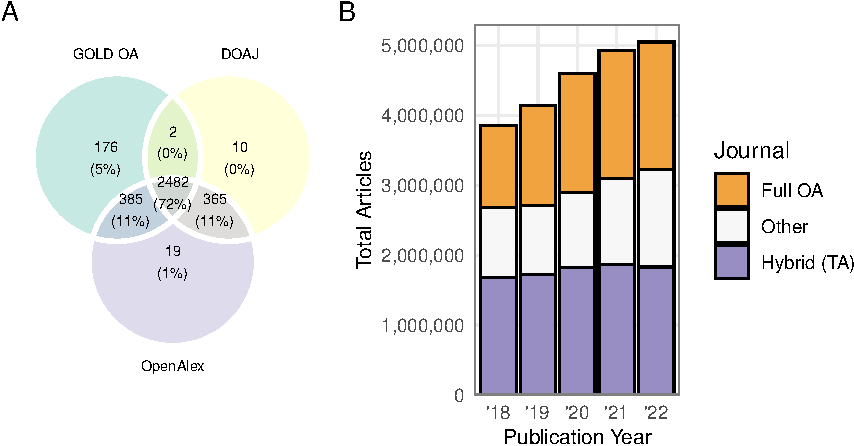
\includegraphics[width=0.99\linewidth]{fig/method_fig-1} \end{center}

\hypertarget{data-analysis}{%
\subsection{Data Analysis}\label{data-analysis}}

\hypertarget{results}{%
\section{Results}\label{results}}

\hypertarget{overview}{%
\subsection{Overview}\label{overview}}

Between 2018 and 2022, a total of 11,189 out of 12,857 hybrid journals
in transformative agreements published at least one open access article
under a Creative Commons license. During this period, these hybrid
journals provided open access to 742,369 out of 8,146,958 articles,
representing a five-year open access proportion of 9.1\%. Authors who
could make use of transformative agreements at the time of publication
contributed 328,957 open access articles to the total.

\begin{figure}

{\centering 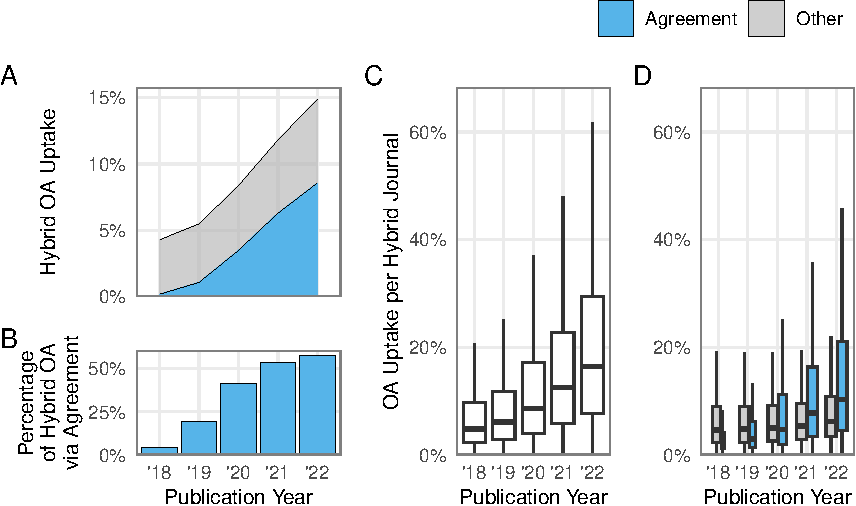
\includegraphics[width=0.99\linewidth]{fig/unnamed-chunk-2-1} 

}

\caption{Relative growth of open access in hybrid journals through transformative agreements between 2018 and 2022 per publication year  according to the total number of articles indexed in Crossref. The blue areas represent open access through transformative agreements, as indicated by the affiliation with institutions that had a corresponding transformative agreement in place at the time of publication according to the first author affiliation data in OpenAlex matched with journal and institutional data from cOAlition S Transformative Agreements Public Data. Grey areas depict open access articles where no link to an agreement could be established. (A) Proportion of open access articles in hybrid journals per year. (B) Percentage of hybrid open access via agreements per year. Boxplots show the proportion of open access articles by individual hybrid journals (C) and individual open access uptake rates by individual hybrid journals and open access funding (D) per publication year. Horizontal lines correspond to the lower quartile, median, and upper quartile, with whiskers extending to ±1.5 of interquartile range. The individual outliers are not shown. Note that data on transformative agreements ending before June 2021 were not available at the time of this study.}\label{fig:unnamed-chunk-2}
\end{figure}

Figure 2A shows a moderate growth in the proportion of open access
articles in hybrid journals, comparing the overall open access uptake
and the impact of transformative agreements on this trend. Over the
five-years period from 2018 to 2022, open access increased from 4.3\% (n
= 65,486) to 15\% (n = 249,511). At the same time, the total article
volume of the investigated journals grew from 1,528,051 in 2018 to
1,676,928 in 2022.

Figure 2B highlights that the majority of open access articles in hybrid
journals were made available through transformative agreements in 2021
and 2022, contributing 58\% of the total open access article volume in
2022. However, there was also a notable growth in open access provision
through individual publication fees, which increased from 4.1\% (n =
62,625) in 2018 to 6.3\% (n = 105,896). This suggests that publishers
were able to gain equally from individual and institutional open access
publishing options.

Figure 2C depicts the substantial variations among the hybrid journals
included in transformative agreements in terms of open access uptake.
Although the median generally follows the trend shown in Figure 2A, the
farther stretch of upper quartiles and whiskers over the years
illustrates that an increasing number of journals published an
above-average proportion of open access articles. In 2022, 25\% of
hybrid journals (n = 2,576) had an open access uptake of 29\%, and 6.6\%
of journals (n = 744) provided the majority of their articles under a
Creative Commons license in the same year. These journals were, on
average, smaller (M = 75, SD = 186) than those with an open access share
below 50\% (M = 164, SD = 347). Notable exception of large journals with
an above-average open access proportion were Physical Review D, a
high-energy physics journal covered by the SCOAP3 consortium that
provided open access to 2,341 out of 4,074 articles in 2022, Astronomy
and Physics (1,396 out of 2,230 articles in 2022 were open access),
which shifted to a subscribe to open business model for all accepted
articles as of April 2022, the Journal of Fluid Mechanics (577 of 1,077
articles in 2022 were open access) and Bioinformatics ( out of articles
in 2022 were open access), which flipped to full open access as of
January 2023.

When comparing the impact of open access trough transformative
agreements across journals, it shows that for many journals these
agreements substantially contributed to the growth of open access over
the years (Figure 2D). Examples of such journals include those with a
scope on specific countries or regions, where also transformative
agreements were implemented. For instance, in 2022, the Germany-based
journals Zeitschrift für Erziehungswissenschaft and Zeitschrift für
Politikwissenschaft, as well as the Scandinavian Political Studies
adressing the Nordic countries, achieved an overall open access uptake
of more than 90\% just through transformative agreements. Despite the
rise in transformative agreements, it is worth noting that other means
of publishing open access in hybrid journals remained common. In total,
9,153 journals published open access articles from authors affiliated
with institutions without transformative agreements in place, while
8,780 journals published at least one open access article through a
transformative agreement in the same year.

\hypertarget{publishing-market}{%
\subsection{Publishing market}\label{publishing-market}}

\begin{table}[H]

\caption{\label{tab:unnamed-chunk-5}Hybrid open access through transformative agreements market shares 2018-2022}
\centering
\fontsize{10}{12}\selectfont
\begin{tabular}[t]{lrllrllrllrll}
\toprule
\multicolumn{1}{c}{ } & \multicolumn{3}{c}{Hybrid journals} & \multicolumn{3}{c}{Articles} & \multicolumn{3}{c}{OA articles} & \multicolumn{3}{c}{TA OA articles} \\
\cmidrule(l{3pt}r{3pt}){2-4} \cmidrule(l{3pt}r{3pt}){5-7} \cmidrule(l{3pt}r{3pt}){8-10} \cmidrule(l{3pt}r{3pt}){11-13}
Publisher & Total & \% & C\% & Total & \% & C\% & Total & \% & C\% & Total & \% & C\%\\
\midrule
Elsevier & 1,936 & 17 & 17 & 2,770,826 & 33.8 & 33.8 & 172,723 & 22.9 & 22.9 & 60,440 & 18.3 & 18.3\\
Springer Nature & 2,274 & 20 & 37 & 1,330,430 & 16.2 & 50 & 175,432 & 23.3 & 46.2 & 100,008 & 30.3 & 48.6\\
Wiley & 1,410 & 12.4 & 49.4 & 1,043,052 & 12.7 & 62.7 & 152,723 & 20.3 & 66.5 & 83,443 & 25.3 & 73.9\\
Other & 5,767 & 50.6 & 100 & 3,061,337 & 37.3 & 100 & 252,523 & 33.5 & 100 & 86,294 & 26.1 & 100\\
\bottomrule
\end{tabular}
\end{table}

Analysing hybrid open access across publishers between 2018 and 2022
reveals a large market concentration. Although 48 publishers offered
transformative agreements, the big three commercial publishers Elsevier,
Springer Nature, and Wiley, accounted for 49\% of total article volume
published (see Table ). Together, they published 500,878 open access
articles, representing 66\% of the open access articles in hybrid
journals. Elsevier, Springer Nature, and Wiley made 243,891 articles
open access in hybrid journals through transformative agreements,
resulting in an even larger market share of 74\%. However, there are
differences among the three large publishers. Although Elsevier
published the largest volume of articles (n = 2,770,826, 34\%), it
published a relatively low number of open access articles, including
those that can be associated with transformative agreements. In
contrast, Springer Nature and Wiley provided open access to a larger
proportion of their articles (13\% of Springer Nature articles and 15\%
of Wiley articles were open acccess), leading to higher open access
market shares (23\% Springer Nature resp. 23\% Wiley). This difference
between Elsevier on the one hand and Springer Nature and Wiley on the
other can be attributed to transformative agreements, as the latter made
the majority of their open access articles available through such deals
(Springer Nature 57\% resp. Wiley 55\%).

\begin{center}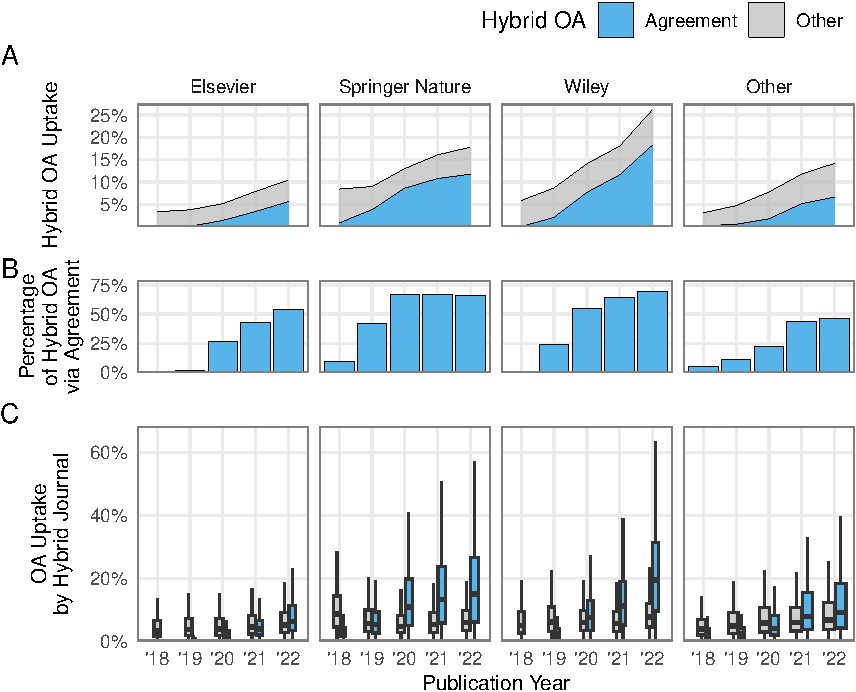
\includegraphics[width=0.99\linewidth]{fig/unnamed-chunk-6-1} \end{center}

Figure 2 takes a closer look into the growth of hybrid open access
across publishers by year with a focus on open articles enabled by
transformative agreements. Although all publishers show a general
long-term trend towards transformative agreements, Figure 2A and 2B
indicate that, in particular, Wiley's has experienced a substantial
increase in its open access share from 5.9\% (n = 11,628) in 2018 to
26\% (n = 53,503) in 2022, rperesenting an 4.5-fold increase. In
contrast, Elsevier's hybrid journals deonstrated a more modest increase,
from 3.3\% (n = 16,872) in 2018 to 10\% (n = 60,821) in 2022, which is a
relatively low open access share compared to the general trend. In 2018,
Springer Nature had the largest open access proportion among the three
publishers of 8.4\% (n = 19,701), but experienced a relatively slower
growth, resulting in 18\% (n = 52,616) of articles being open access in
Springer Nature hybrid journals in 2022.

The varying degrees of uptake of open access across the three major
publishers can be attributed to distinct approaches to transformative
agreements. Springer Nature, for example, began in 2015 offering
selected consortia, such as the Max Planck Society, the Swedish Bibsam
consortium, and the Finnish FinELib consortium, open access agreements
for its hybrid journal portfolio under the name Springer
Compact\footnote{\url{https://web.archive.org/web/20180414062853id_/http://www.liber2015.org.uk/wp-content/uploads/2015/03/Springer-Compact.pdf}}.
However, these agreements were not included in the data as they
concluded prior to the start of the transformative agreement data
collection in June 2021. Nonetheless, the results suggest the importance
of central agreements for Springer Nature's hybrid open access business
over the past five years (Figure 2B). In 2022, 66\% (n = 34,725) of open
access articles in f Springer Nature hybrid journals were enabled
through transformative agreements. In the same year, 70\% (n = 37,316)
of Wiley's open access articles could be linked to transformative
agreements in 2022. In contrast, Elsevier published fewer than half of
its open access articles through transformative agreements (n = 32,627;
54\%).

The increasing trend towards transformative agreements can be also
observed at the journal-level (Figure 2). While no substantial
differences between open access enabled through transformative
agreements and other revenue source could observed across Elsevier
journals, the distribution of open access across Springer Nature and
Wiley hybrid journals indicates that the growth is not limited to a few
journals, but extends across the portfolio. In particular, Wiley's upper
quantile, which represents the top 25\% of journals in terms of the
proportion of open access articles from transformative agreements,
increased markedly from 13\% in 2020 to 31\% in 2022. At the same time,
the median proportion grew from 7.5\% to 19\%. It is interesting to note
that a small but increasing number of journals from these two publishers
are providing open access to the majority of articles through
transformative agreements. Wiley recorded 68 and Springer Nature 102
hybrid journals with an open access share above 50\% that could be
solely attributed to transformative agreements. Upon inspection, these
journals were mainly society or local language journals with a small
yearly article volume.

\hypertarget{journal-subjects}{%
\subsection{Journal subjects}\label{journal-subjects}}

Table presents a high-level overview of hybrid open access by AJCS
subject area using fractionalised counting to account for journals
belonging to more than one category. Between 2018 and 2022, most hybrid
journals with at least one open articles could be attributed to the
social sciences including the humanities. However, these journals
published the fewest number of articles, whereas physical sciences
journals recorded most articles, followed by the health sciences and the
life sciences. In terms of open access, physical sciences journals
accounted for more than one third of articles published in the
five-years period, followed by the health science, the social sciences
and the life sciences.

\begin{table}[H]

\caption{\label{tab:subject_summary_table}Hybrid open access through transformative agreements by journal subject 2018-2022}
\centering
\begin{tabular}[t]{lrllrllrllrll}
\toprule
\multicolumn{1}{c}{ } & \multicolumn{3}{c}{Hybrid journals} & \multicolumn{3}{c}{Articles} & \multicolumn{3}{c}{OA articles} & \multicolumn{3}{c}{TA OA articles} \\
\cmidrule(l{3pt}r{3pt}){2-4} \cmidrule(l{3pt}r{3pt}){5-7} \cmidrule(l{3pt}r{3pt}){8-10} \cmidrule(l{3pt}r{3pt}){11-13}
Journal subject & Total & \% & C\% & Total & \% & C\% & Total & \% & C\% & Total & \% & C\%\\
\midrule
Health Sciences & 2,376 & 22.5 & 22.5 & 2,709,906 & 27.8 & 27.8 & 286,592 & 27.3 & 27.3 & 117,746 & 25 & 25\\
Life Sciences & 1,403 & 13.3 & 35.8 & 1,477,808 & 15.1 & 42.9 & 191,880 & 18.3 & 45.6 & 71,593 & 15.2 & 40.2\\
Physical Sciences & 2,732 & 25.9 & 61.7 & 4,291,833 & 44 & 86.9 & 366,794 & 35 & 80.6 & 167,686 & 35.6 & 75.8\\
Social Sciences & 4,050 & 38.3 & 100 & 1,280,460 & 13.1 & 100 & 203,461 & 19.4 & 100 & 114,190 & 24.2 & 100\\
\bottomrule
\end{tabular}
\end{table}

Figure presents the relative growth of hybrid open access by subject
area between 2018-2022. In particular, Social Sciences and Humanties
journals accounted for the strongest growth in the five-years period
from 6.4\% (n = 8,361) to 23\% (n = 51,938), followed by the Life
Science from 7.6\% (n = 15,003) to 18\% (n = 39,494) , Health Science
from 5.3\% (n = 18,279) to 16\% (n = 63,089) and Physical Sciences from
4.5\% (n = 22,364) to 12\% (n = 85,428). This growth in the social
sciences can be largely attributed to transformative agreements. In
2022, two-third of open access articles (67\%, n = 34,759) were
published by first authors affiliated with participating institutions.
Figure C shows that this trend is consistent across Social Sciences
journals. In 2022, 25\% of Social Science journals provided open access
to at least every fourth article exclusively through transformative
agreements. However, hybrid open access through transformative
agreements played a comparable lesser role in the Life Sciences and
Health Sciences. In these two subject areas, only about half of the open
access articles can be linked to these agreements, both overall and on
median average across journals. In contrast, the majority of Physical
Science Journals, shows an increase of open access through
transformative agreements compared to other options to publish open
access in hybrid journals.

\begin{center}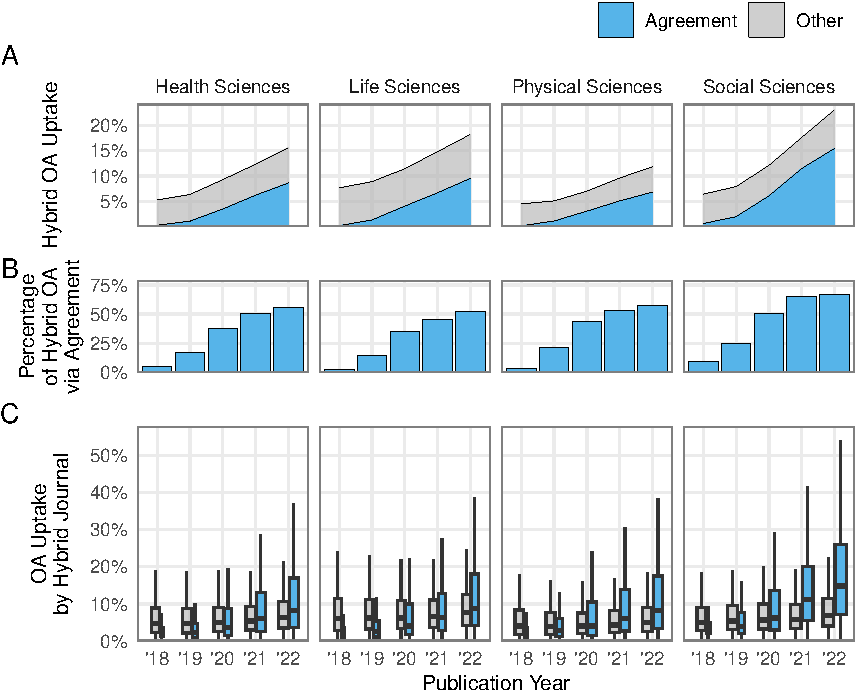
\includegraphics[width=0.99\linewidth]{fig/subject_panel-1} \end{center}

\hypertarget{comparing-countries}{%
\subsection{Comparing countries}\label{comparing-countries}}

Between 2018 and 2022, Western economies almost exclusively dominated
hybrid open access publishing through transformative agreements. During
this period, first-authors affiliated with institutions from
Organisation for Economic Co-operation and Development (OECD) member
countries published 602,050 open access articles in hybrid journals,
representing 81\% of the investigated open access articles. This
disparity between OECD nations and other countries becomes even more
evident when considering open access through transformative agreements,
as 310,712 of 328,957, or 94\% of open access articles were associated
with such agreements.

\begin{center}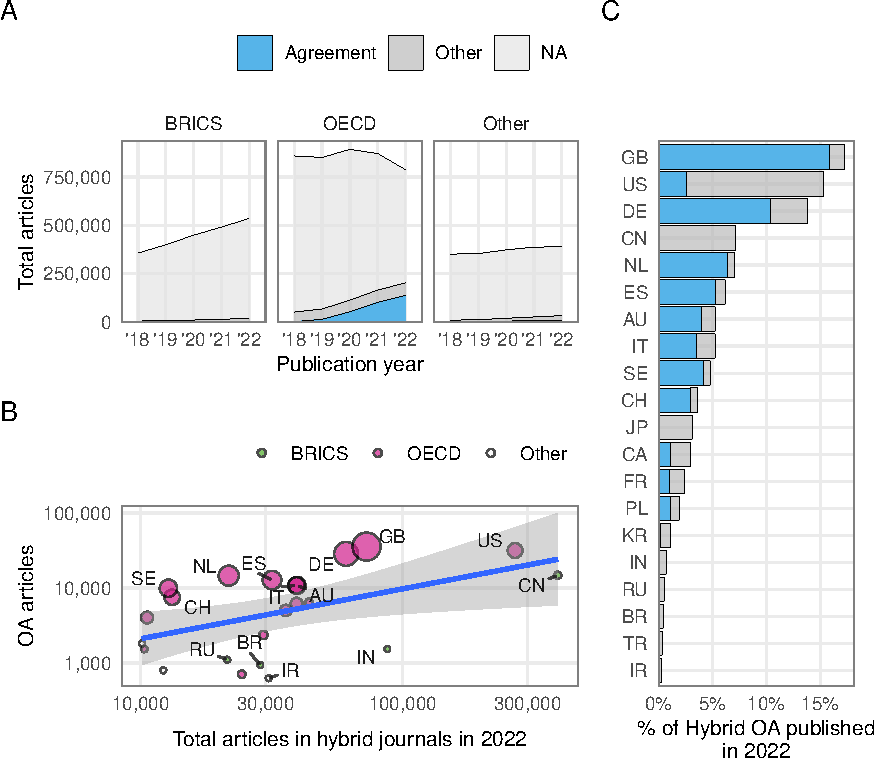
\includegraphics[width=0.99\linewidth]{fig/country_patch-1} \end{center}

Figure 2A shows the development of hybrid open access publishing by
countries, comparing the OECD area with the BRICS, an intergovernmental
organisation, which comprised the countries Brazil, Russia, India, China
and South Africa in 2022. The residual category ``Other'' includes the
remaining countries. From 2018 to 2022, the proportion of open access in
hybrid journals increased from 6.1\% in 2018 to 26\% in 2022. On the
other hand, BRICS recorded an low uptake, from 1.6\% in 2018 to 3.7\% in
2022.\\
Despite rise of open access across OECD countries, the overall
publication output decreased sharply, dropping to 786,903 in 2022 after
peaking 892,197 articles in 2020. In stark contrast, the number of
articles published in hybrid journals by first authors affiliated with
institutions from BRICS countries increased steadily over the years,
more than doubling from 356,632 in 2018 to 786,903 in 2022. Upon closer
examination, this trend can be observed across all big three publishers,
although the shift towards BRICS is particularly evident in Elsevier's
hybrid journal portfolio, in particular with regard to articles
published in Physical Sciences journals (see Supplement). While OECD
publication output in Elsevier's Physical Sciences journals declined
from 112,822 articles in 2018 to 103,766 in 2022, BRICS output increased
from 104,654 to 171,713 in the same five-year period. Furthermore, OECD
publication output in Health Science Journals and Life Science journals
stagnated across the investigated hybrid journal portfolios after a peak
in 2020.

To illustrate the situation in 2022, Figure B compares total publication
output with the number of open access articles. With 391,530 articles,
China was the most productive country, followed by the United States
(268,965 articles) and India (87,428 articles). In contrast, West and
Nord European countries published a considerable high number of open
access articles, mainly due to transformative agreements. Particularly,
Germany, Great Britain, the Netherlands, Sweden, Switzerland and Spain
recorded an above-average open access share as indicated by the linear
trend line. As represented by the point size, as well as it can been
seen in Figure C, transformative agreements contributed to this market
position of these countries. Interestingly, the United States had a
notable open access market share of 15\%, although transformative
agreements contributed to a lesser extent. Similarly, China's open
access market share of 7.2 in 2022 was comparable to that of the
Netherlands, which was (7.1\%,).

\begin{center}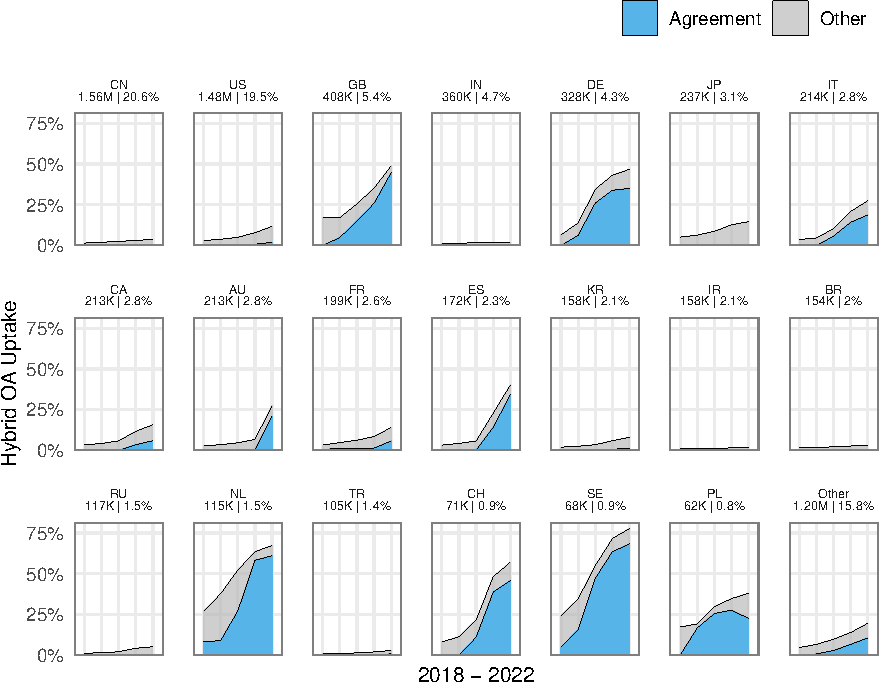
\includegraphics[width=0.99\linewidth]{fig/country_top_20_plot-1} \end{center}

Figure illustrates the development of hybrid open access from 2018 to
2022, highlighting the top 20 most productive countries in terms of
articles published in hybrid journals that were included in
transformative agreements over the five-year period. Notably, The
Netherlands (27\%), Sweden (24\%), Poland (17\%) and Great Britain
(17\%)) exhibited a relatively high level of uptake in 2018 which
continued to increase in the following years. In 2022, Sweden had the
highest proportion of open-access articles relative to its publication
output (78\%), followed by the Netherlands (67\%) and Switzerland
(57\%), with these countries benefiting from transformative agreements.
In Germany, however, hybrid open access only began to increase from 2019
onwards after the successful negotiation of nationwide agreements with
Wiley (July 2019) and Springer Nature (January 2020). Prior to this,
only a few organisations had agreements in place, for the example the
Max Planck Society with Springer Compact.

Since 2021, there has been a general trend towards hybrid open access
among many western countries, primarily driven by transformative
agreements. However, proliferation of transformative agreements differe
across these countries. For instance, Germany successfully negotiated an
agreement with Elsevier not until 2023. Additionally, publication limits
or eligibility criteria for institutions and article types may explain
why even countries with widespread agreement implementation do not
achieve 100\% hybrid open access. Interestingly, in Japan and the US
other options than transformative agreements were the main driver for
the increase in hybrid open access. Once again, the graph highlights
countries with low hybrid open access, particularly non-OECD countries,
where only a few or no agreements were in place.

\hypertarget{supplements}{%
\subsubsection{Supplements}\label{supplements}}

\begin{center}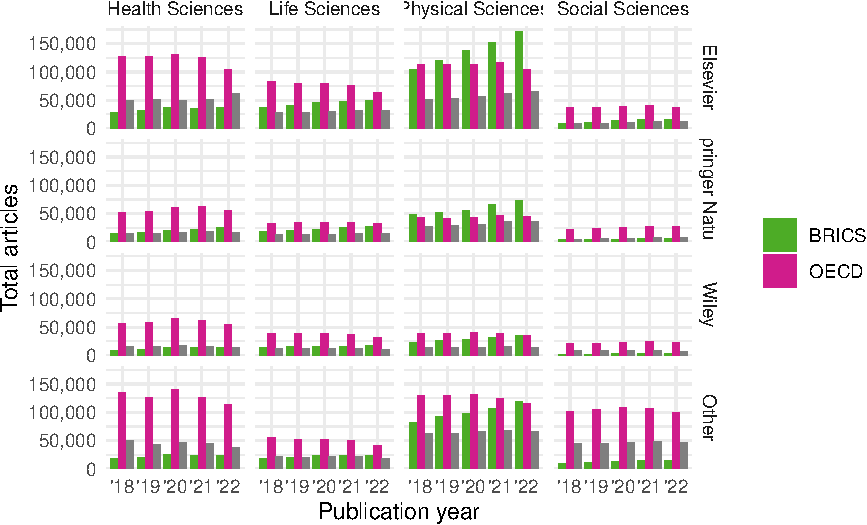
\includegraphics[width=0.99\linewidth]{fig/unnamed-chunk-10-1} \end{center}

\hypertarget{refs}{}
\begin{CSLReferences}{1}{0}
\leavevmode\vadjust pre{\hypertarget{ref-Borrego_2020}{}}%
Borrego, Á., Anglada, L., \& Abadal, E. (2020). Transformative
agreements: Do they pave the way to open access? \emph{Learned
Publishing}. \url{https://doi.org/10.1002/leap.1347}

\leavevmode\vadjust pre{\hypertarget{ref-goldoa}{}}%
Bruns, A., Cakir, Y., Kaya, S., \& Beidaghi, S. (2022).
\emph{{ISSN-Matching of Gold OA Journals (ISSN-GOLD-OA) 5.0}}. Bielefeld
University. \url{https://doi.org/10.4119/unibi/2961544}

\leavevmode\vadjust pre{\hypertarget{ref-Geschuhn_2017}{}}%
Geschuhn, K., \& Stone, G. (2017). It's the workflows, stupid! What is
required to make {``offsetting''} work for the open access transition.
\emph{Insights the {UKSG} Journal}, \emph{30}(3), 103--114.
\url{https://doi.org/10.1629/uksg.391}

\leavevmode\vadjust pre{\hypertarget{ref-Larivi_re_2016}{}}%
Larivière, V., Desrochers, N., Macaluso, B., Mongeon, P., Paul-Hus, A.,
\& Sugimoto, C. R. (2016). Contributorship and division of labor in
knowledge production. \emph{Social Studies of Science}, \emph{46}(3),
417--435. \url{https://doi.org/10.1177/0306312716650046}

\leavevmode\vadjust pre{\hypertarget{ref-Schimmer_2015}{}}%
Schimmer, R., Geschuhn, K., \& Vogler, A. (2015). \emph{{Disrupting the
subscription journals'business model for the necessary large-scale
transformation to open access}}. Max Planck Digital Library.
\url{https://doi.org/10.17617/1.3}

\end{CSLReferences}

\end{document}